\documentclass[12pt]{support/thcolognethesis} 

\usepackage{amssymb}

\title{Optimierung von Augmented Reality Anwendungen durch die Berücksichtigung von Tiefeninformationen mit Googles Project Tango}

\degree{Masterthesis}

\author{Steffen Tröster}

\college{
	Technischen Hochschule Köln\\
    Ingenieurwissenschaftliches Zentrum\\
    Fakultät für Informations-,\\
    Medien- und Elektrotechnik}

\course{Technische Informatik (Master)}

\company{inovex GmbH}  

\firstExaminer{Prof. Dr. Martin Eisemann}
\firstExaminerLocation{Technische Hochschule Köln}
\secondExaminer{Christian Meder}
\secondExaminerLocation{inovex GmbH}

\degreedate{Köln, im \monthyeardate\today}
	
\begin{document}

\baselineskip=18pt plus1pt

\setcounter{secnumdepth}{3}
\setcounter{tocdepth}{3}

\maketitle                 

\begin{abstract}
\setlength{\parskip}{1em}

Project Tango ist eine neue mobile Plattform des Google Advanced Technology and Project (ATAP) Teams, die in der Lage ist, Bewegungsverfolgung, Tiefenwahrnehmung und Umgebungswiedererkennung auf Smartphones und Tablets anbieten zu können. Durch die kontinuierliche Bestimmung der relativen Geräteposition eignet sich die Plattform besonders für dreidimensionale Augmented Reality (AR) Anwendungen. Die Illusion dieser AR Anwendungen wird besonders dann gestört, wenn sich reale Objekte in einer Szene räumlich vor virtuellen Objekten befindet und diese virtuellen Objekte nicht entsprechend ausgespart werden. 

Diese Arbeit stellt daher drei Überdeckungsverfahren vor, mit denen diese Überlagerung der virtuellen Objekte mit Hilfe der Tiefenwahrnehmung von Project Tango und des Z-Buffer Algorithmus realisiert werden kann. Die Tiefeninformationen für den Z-Buffer werden hierfür zum einen direkt aus den Sensordaten und alternativ mit einer TSDF Rekonstruktion und einer selbst zusammengestellten Ebenen Rekonstruktion bestimmt. Außerdem wird auf einen zusätzlichen Ansatz eingegangen, der zur Verbesserung dieser Tiefeninformationen die Bildinformationen der Farbkamera durch den Guided Filter berücksichtigt. Diese Mechanismen werden im Laufe der Arbeit prototypisch umgesetzt und gegenübergestellt. 

\setlength{\parskip}{0em}
\end{abstract}
\selectlanguage{english}
\begin{abstract}
\setlength{\parskip}{1em}

Project Tango is a new mobile platform by Google’s Advanced Technology and Projects (ATAP) Teams, which brings Motion Tracking, Depth Perception, and Area Learning to mobile devices. With Project Tango, Google is providing a technology to tablets and smartphones for building virtual reality (VR), indoor navigation, precise measurement and augmented reality applications. The focus of this document lies mainly upon augmented reality applications. Although you can build an effective 3D AR illusion with the continuous device motion tracking, there is still a problem, that the scenes virtual object cannot be occluded by real objects when they are in foreground.

Since the Project Tango platform is offering a continues depth perception of the current viewport, this depth information can be used to solve the missing occlusion issue. This work is introducing three approaches to enable an augmented reality occlusion by real objects. Additionally an approach will be discussed to optimize the depth occlusion by taking the color information by the device’s camera into account. These methods will also get implemented with the development kit, tested, compared and evaluated concerning their applicability.

\setlength{\parskip}{0em}
\end{abstract}
\selectlanguage{ngerman}


         

\begin{romanpages}         
\tableofcontents            
\end{romanpages}          

\chapter{Einleitung}

Project Tango ist eine neue mobile Plattform des Google Advanced Technology and Projects (ATAP) Teams, welche Bewegungsverfolgung, Tiefenwahrnehmung und Umgebungswiedererkennung auf mobilen Endgeräten realisiert.

\begin{quotation}
\enquote{Project Tango combines 3D motion tracking with depth sensing to give your mobile device the ability to know where it is and how it moves through space.}  \citep{Proje19:online}
\end{quotation}

Diese Verfügbarkeit dieser Echtzeitdaten ermöglicht viele verschiedene neue Einsatzmöglichkeiten auf mobilen Endgeräten wie Smartphones und Tablets. Typische Einsatzszenarien dieser Plattform sind die Indoor Navigation, die Vermessung der Umgebung sowie andere Anwendungen im Bereich Virtual und Augmented Reality. Der Fokus dieser Forschungsarbeit liegt hier in dem Anwendungsbereich der dreidimensionalen Augmented Reality (AR). 

Die Anwendungsgebiete für Augmented Reality (dt. Erweiterte Realität) sind sehr vielseitig und liegen in der Medizin, der Unterhaltungsindustrie, Bildung und in vielen weiteren Industriezweigen. Eine barrierefreie Navigationshilfe, Einblendungen für die persönliche Assistenz, kontextsensitive Projektionen und Computerspiele sind Beispiele für typische Anwendungen, die durch AR umgesetzt werden können. 

Für die erfolgreiche Umsetzen einer Augmented Reality Anwendung, müssen die Kameraeigenschaften, wie Brennweite, Verzerrung und die Position der Kamera zu jeder Zeit und idealerweise in Echtzeit bekannt sein. Sensoren wie Kompass, INS (Trägheits\-navigations\-system) oder GPS können zwar eine grobe Lokalisierung ohne bekannte Merkmale im Raum ermöglichen, führen aber langfristig zu Fehlern, wenn keine optischen Referenzen gegeben sind. Mit Hilfe von der Bewegungsverfolgung durch Project Tango kann diese Lokalisierung der Kamera und somit die korrekte Positionierung von virtuellen Objekten im Raum deutlich zuverlässiger, in Echtzeit und ohne vordefinierte Merkmale im Raum realisiert werden. Project Tango eignet sich daher sehr gut für die Umsetzung und den Einsatz von AR Anwendungen.

\section{Augmented Reality Optimierung}

Um eine für den Betrachter effektive und optimierte Augmented Reality Anwendung umsetzen zu können, benötigt man laut \citet{azuma2001recent} die Möglichkeit mehr Informationen über relevante Objekte im realen Raum ermitteln zu können. Durch diese Informationen könnte dem Nutzer zum Beispiel eine Interaktion mit realen Objekten ermöglicht werden oder anhand optischer und semantischer Einordnung der Umgebung passende Funktionen angeboten werden. 

Hinsichtlich der zuletzt erwähnten Kontextsensitivität existieren viele Ansätze, basierend auf optischen Merkmalen der Umgebung. So kann zum Beispiel ein optisches Tracking von realen Objekten, wie von \citet{lee2008hybrid} beschrieben, umgesetzt werden. Project Tango nutzt bereits optische Merkmale, um eine Positionsverfolgung oder das Lernen der Umgebung umzusetzen. Wären diese Merkmale für den Entwickler als Schnittstelle verfügbar, könnte man mit diesen Informationen solche kontextsensitiven Anwendungen umsetzen. Der Fokus soll in dieser Arbeit jedoch nicht auf den optischen Merkmalen sondern auf den Tiefeninformationen, die Project Tango durch den eingebauten Tiefensensor in Form einer Pointcloud liefern kann, liegen.

Ein sinnvoller Einsatz von Augmented Reality Anwendungen besteht darin, virtuelle Objekte in eine echte Szene zu projizieren. Dabei überlagert die Projektion des virtuellen Objekts das aktuelle Kamerabild oder den aktuellen Sichtbereich und erwirkt dadurch den Anschein, als ob sich das virtuelle Objekt wirklich in der Szene befindet. Dieser Effekt funktioniert solange erfolgreich, bis ein reales Objekt sich räumlich vor das virtuelle Objekt bewegt und die zu erwartende Überlagerung des virtuellen Objekts nicht erfolgt. Diese fehlerhafte Darstellung durch eine fehlende Überdeckung ist in Abbildung \ref{fig:occlusion-problem} zu erkennen. 

\begin{figure}[h]
  \centering
	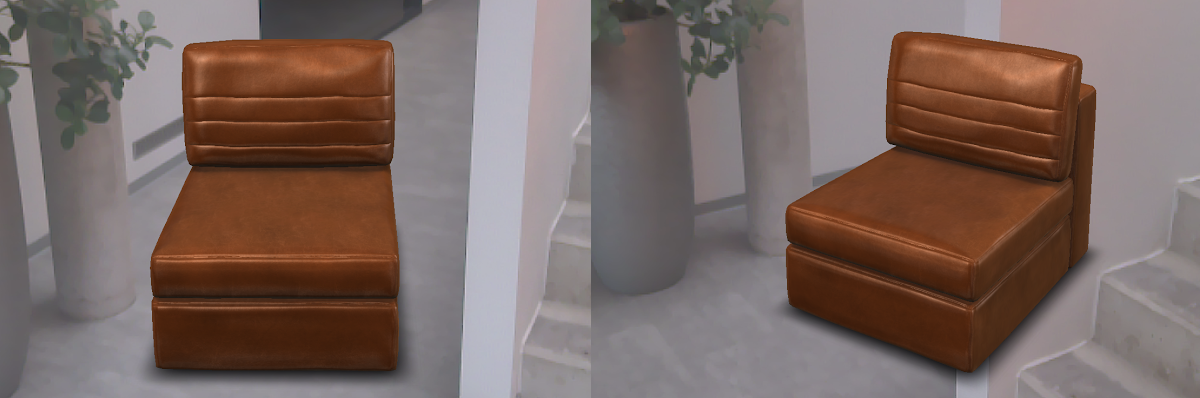
\includegraphics[width=1.0\textwidth]{content/images/occlusion-problem.png} 

  \caption{AR Projektion mit Project Tango - Links: Erfolgreiche Projektion. Rechts: Fehlerhafte Darstellung ohne Überdeckung.}
  \label{fig:occlusion-problem}
\end{figure}

Die Verfügbarkeit der Tiefeninformationen bei Project Tango könnte die Interaktionen oder Darstellungen in einer Augmented Reality Anwendung präziser an die echten räumlichen Gegebenheiten anpassen. Es existieren zum Beispiel prototypische Anwendungen, in denen virtuelle Markierungen passend an echten Objekten im virtuellen Raum positioniert werden können, indem sie auf die aktuellen Tiefeninformation des Sichtbereichs zurückgreifen. Eine weitere Idee ist es, Überlagerungen virtueller Objekte ermitteln zu können, an denen sich reale Objekte im Vordergrund befinden.

\section{Zielsetzung und Vorgehen}

Diese Arbeit will die Fragestellung beantworten, durch welche Verfahren mithilfe der Tiefeninformationen von Project Tango, automatisch und in Echtzeit die Überdeckung virtueller Objekte mit realen Objekten in einer Augmented Reality Szene realisiert werden kann. Dabei soll Project Tango als autonomes System betrachtet werden, welches diese Problemstellung selbstständig und mit den eingeschränkten Ressourcen dieser mobilen Plattform lösen soll.

Hierzu sollen zunächst bestehende Verfahren zur Bestimmung einer Augmented Reality Überdeckung durch eine Literaturrecherche gefunden werden. Diese Verfahren sollen dabei auf Ihre Anwendbarkeit mit der Project Tango Hardware überprüft werden. Sollten sich aus der Recherche weitere Ideen ergeben, wie speziell auf der Project Tango Hardware eine Überdeckung umgesetzt oder verbessert werden kann, sollen diese mit in die Arbeit eingebunden werden. Eine Idee könnte zum Beispiel sein, auch das Farbbild der normalen Kamera von Project Tango in die Optimierung der virtuellen Überlagerung einfließen zu lassen. Die identifizierten Verfahren sollen hiernach entsprechend implementiert werden, um sie darauf folgend in einer Testumgebung gegenüber zu stellen.

Strukturell wird in dieser Arbeit in Kapitel \ref{sec:thema} erst einmal auf die thematischen Grundlagen zu Augmented Reality und Project Tango eingegangen. Hier werden auch die existierenden Verfahren zur AR Überdeckung angesprochen. Unter Kapitel \ref{sec:algorithms} sind theoretische Grundlagen zu finden, die bei der späteren Umsetzung verschiedener Verfahren angewendet werden. Kapitel \ref{sec:optimization} beinhaltet die Argumentation und Beschreibung der gewählten Verfahren, welche unter Kapitel \ref{sec:implementation} auf der Project Tango Hardware umgesetzt werden. In Kapitel \ref{sec:evaluation} werden die vorliegenden Umsetzung in einem Testszenario gegenübergestellt, um eine Aussage treffen zu können, welcher Ansatz auf der Hardware oder für einen bestimmten Einsatz gut funktionieren könnte.



\chapter{Theoretische Vorbemerkung}

Im ersten Teil dieses Kapitels werden zunächst einmal die Grundlagen zu Augmented Reality beschrieben, wie diese Technologie einzuordnen ist, welche technischen Anforderungen ein Augmented Reality System hat und wo typische Einsatzszenarien liegen.


\section{Augmented Reality}

Augmented Reality (AR) ist eine Klasse aus dem Realitäts-Virtualitäts-Kontinuum von \cite{milgram1995augmented}, zu finden in Abbildung \ref{fig:virtual-continuum}, welche reale und virtuelle Objekte in einer realen Umgebung kombiniert. Diese virtuellen Objekte sind in der realen Umgebung idealerweise fest lokalisiert und fügen sich somit in das reale Erscheinungsbild ein. Typischerweise sind AR Anwendungen interaktiv, und stellen die virtuellen Objekte in Echtzeit und dreidimensional in der realen Welt dar. Für die Definition von AR Anwendungen gibt es zudem keine Limitierung für die Darstellungstechnologie, wie zum Beispiel das Projekt Tango Tablett oder einem Head-Mounted Display. AR beschränkt sich zudem nicht auf den angesprochenen Sinn - so sind zum Beispiel AR Anwendungen mit visueller, taktiler oder sogar olfaktorischer Umsetzung möglich.\\

Virtuel Reality (VR) oder auch Virtual Environment hingegen kapselt sich von der realen Umgebung ab und bietet Interaktionen in reinen virtuellen Umgebungen. VR konnte sich im Gegensatz zu AR deutlich schneller Entwickeln, da die technologischen Anforderungen an AR deutlich höher sind. \citep{van2010survey}\\

\begin{figure}
  \centering
	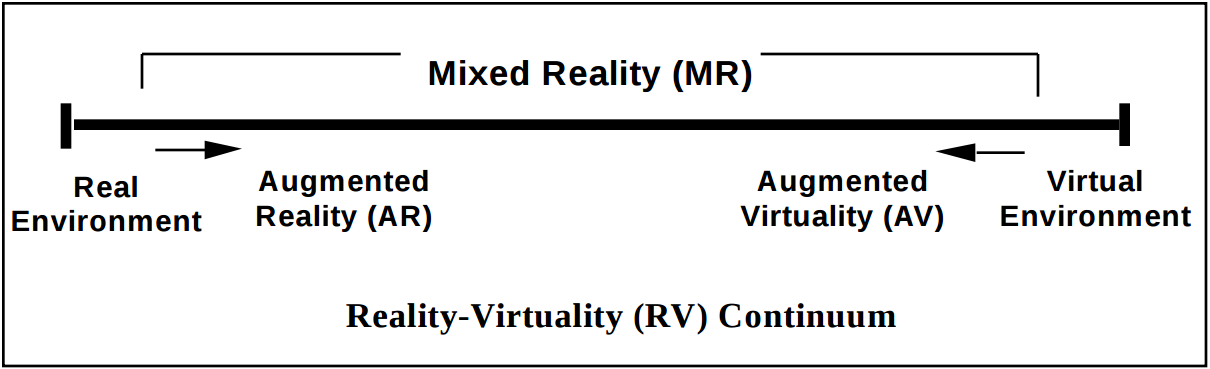
\includegraphics[width=0.85\textwidth]{content/images/theory/virtual-continuum.png} 
  \caption{Vereinfachte Darstellung des Realitäts-Virtualitäts-Kontinuum von \citet*{milgram1995augmented}}
  \label{fig:virtual-continuum}
\end{figure}

\subsection{Technische Anforderungen}

Dieser Abschnitt widmet sich den technischen Anforderungen an Augmented Reality, indem die potentiellen Display Technologien beschrieben werden, mögliche Trackingverfahren erläutern werden und zuletzt die Systeme bestimmt werden, mit denen ein Nutzer mit dem AR System interagieren kann.\\

\subsubsection{Display Technologie}

Der erste wichtige Teil der technologischen Anforderungen an AR sind visuelle Anzeigen (visual displays), welche sich nach \citet{van2010survey}
in diesem Anwendungsfall zunächst in drei Arten der Darstellung unterteilen und zudem unterschiedlich positioniert werden können. Die einfachste und günstigste Art der visuellen Darstellung in AR ist \enquote{video see-through}, wodurch die reale Umgebung durch eine Video Aufnahme ersetzt wird und die virtuellen Objekte digital in die Video Aufnahme gerendert werden. Das bietet außerdem die Möglichkeit Objekte aus der realen Umgebung zu entfernen oder zu ändern oder anhand der Luminanz Information vom Video das Rendering der virtuellen Objekte entsprechend an die Realität anzupassen.\\

Die nächste Möglichkeit zur Darstellung ist \enquote{optical see-through}, wodurch die virtuellen Objekte durch transparente Spiegel in das Sichtfeld des Betrachters gebracht werden. Anders als bei \enquote{video see-throught} bleibt die reale Auflösung für die visuelle Aufnahme des Betrachtes gleich und es können zudem keine Latenzprobleme beim Ändern des Betrachtungswinkels auftreten (parallax-effect).\\

Die dritte Möglichkeit ist die projizierte Darstellung, in der die Augmented Reality Überlagerung auf die realen Objekte projiziert werden. Diese Darstellung ermöglicht die Abdeckung vom gesamten Sichtfeld, benötigt aber eine entsprechende Kalibrierung bei Umgebungsänderungen.\\

Neben der Art der Darstellung können die Display Technologien laut \citet{azuma2001recent} anhand Ihrer Positionierung klassifiziert werden. Man unterscheidet zwischen am Kopf befestigten Displays (head-mounted), tragbare Displays (hand-held) und räumlich positionierten Displays. Zu jeder dieser Displayarten gibt es wiederum unterschiedliche technische Umsetzungen mit ihren spezifischen Vor- und Nachteilen bezüglich ihrer Anwendungsszenarien.\\

\subsubsection{Tracking Technologien}

Um eine virtuelle Projektion im realen Raum zu realisieren muss zunächst die Position und gegebenenfalls relative Positionsänderung des Displays bestimmt werden, auch \enquote{augmented reality registration} genannt. Man spricht dabei üblichweise von den \enquote{six degrees of freedom (6DOF)}, der Position im Raum (x, y, z) und der Orientierung (yaw, pitch, roll). \\

Frühe Techniken für die Registrierung benötigten üblicher Weise eine speziell vorbereitete Räumlichkeit, denn sie basierten auf mechanischen, magnetischen oder Ultraschall Sensoren um die Position zu bestimmen. Diese Sensoren sind zwar immer noch im Einsatz und bilden auch den Grundstein für AR und VR Forschung, sind aber praktisch gesehen zu komplex und aufwändig für die meisten Anwendungsfälle. \citep{van2010survey} \\

Für ein grobes Positions-Tracking, vor allem auch außerhalb von Gebäuden wird GPS genutzt. Für großräumliche Anwendung ist GPS, mit einer Varianz von 10-15 Metern und in Kombination mit einem Kompass, durchaus praktikabel. Zum Beispiel um sichtbare Flugzeuge oder Sterne visuell aufzubereiten. Innerhalb von Gebäuden basiert die grobe Positionierung laut \citet{van2010survey} oft auf verfügbaren Wifi Access Points oder RFID Markern. \citet{lamarca2005place} demonstrieren hierzu auch die Möglichkeit diese Technologie für grobe Lokalisation außerhalb von Gebäuden einzusetzen.\\

Optische Tracking Verfahren basierend auf Bildverarbeitung bieten laut \citet{van2010survey} deutlich genauere Resultate als die zuvor beschriebenen Verfahren. Es gibt hier viele verschiedene sensorische Ansätze ein optisches Tracking zu realisieren. Frühe verfahren nutzten referenzielle Marker oder Licht emittierende LEDs in einem vordefinierten Modell, um zwischen aufgenommenen Bildern eine homographische Transformation zu berechnen und um somit Rückschlüsse auf die Rotation und Positionsänderung der Kamera zu ziehen. Neue Verfahren ohne Marker nutzen Techniken zur Feature Detection und Matching um Referenzen und Bewegungen zwischen aufgenommenen Bildern zu bestimmen.\\

Viele kommerzielle und erfolgreiche Tracking Verfahren beruhen jedoch auf hybride Ansätze indem Sensoren kombiniert werden um potentielle Fehleinschätzungen eines Sensors oder einer Technik auszuschließen. So werden zum Beispiel Neigungssensor, Kompass und Gyroskop mit einem optischen Verfahren kombiniert um ein Tracking der sechs Freiheitsgrade zu optimieren. \citep{van2010survey}\\

\citet{azuma2001recent} erwähnt an dieser Stelle auch die Kalibrierung der Sensoren, die für ein präzises Registrieren nötig ist. So müssen zum Beispiel die Linseneigenschaften der Kamera für optisches Tracking bekannt sein, damit die Verfahren mit Krümmungen oder Verzerrungen umgehen können. Diese Informationen sind auch bei video see-through Displays für ein korrektes Projezieren der 3D Objekte wichtig. Zudem wird erwähnt, dass man Messfehlern oder Drifts der Position zum Beispiel mit der Zunahme von Gyroscop Informationen entgegenwirken kann, indem man auf Ereignisse wie einen Schritt des Nutzers wartet. \citep{azuma2001recent} \\

\subsubsection{Interaktions Technologien}

*

\subsection{Anwendungsbereiche}

* 


\appendix
\listoffigures            
\include{content/acknowlegements}
\chapter{Ergebnisaufnahmen}
\begin{sidewaysfigure}[h]
  \centering
	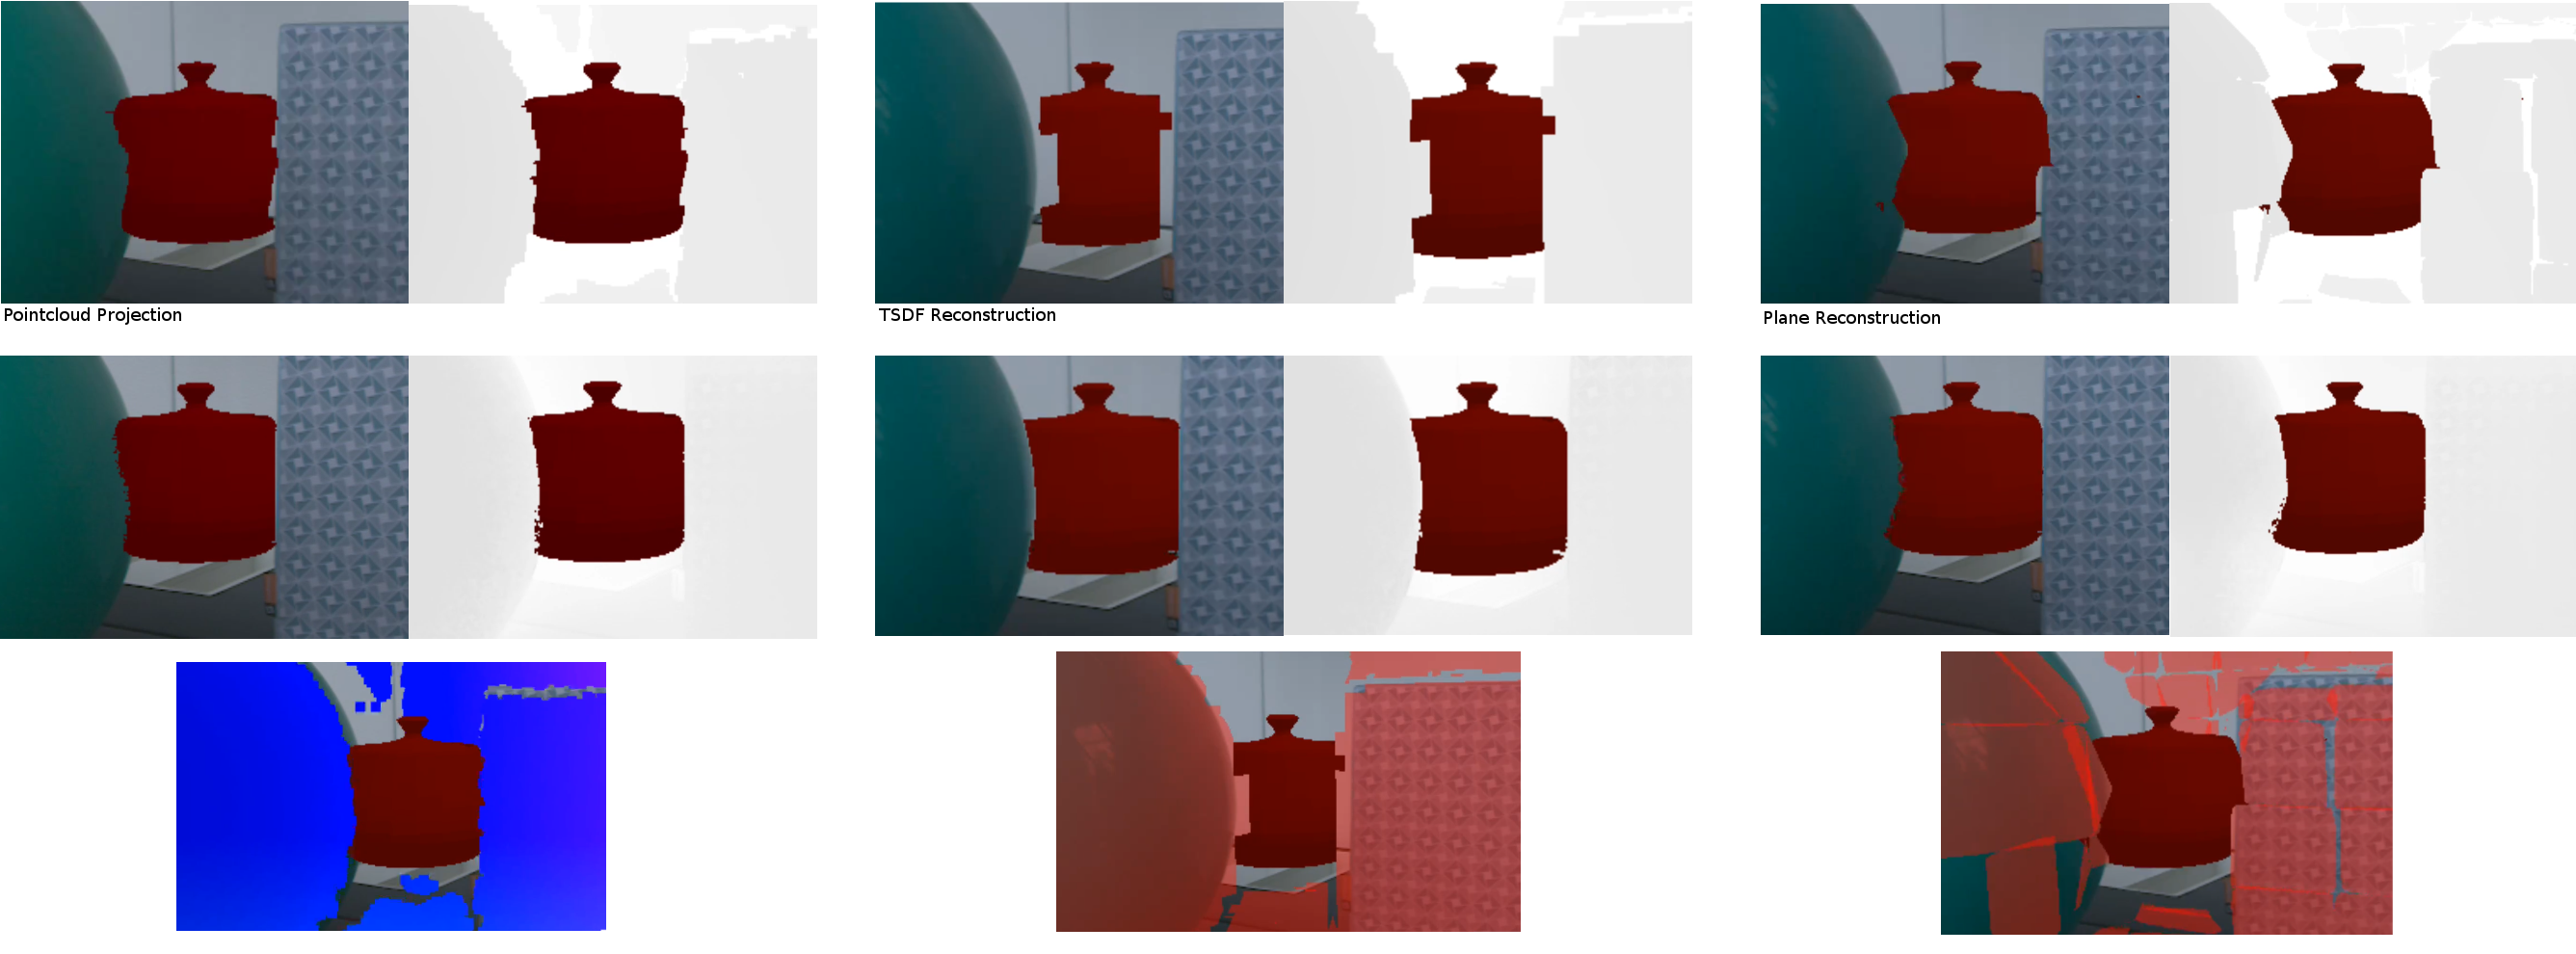
\includegraphics[width=1.0\textwidth]{content/images/evaluation/static_occlusion.png} 
  \caption{Ergebnisaufnahmen aus der ersten statischen Szene}
  \label{fig:static_occlusion}
\end{sidewaysfigure}

\begin{sidewaysfigure}[h]
  \centering
	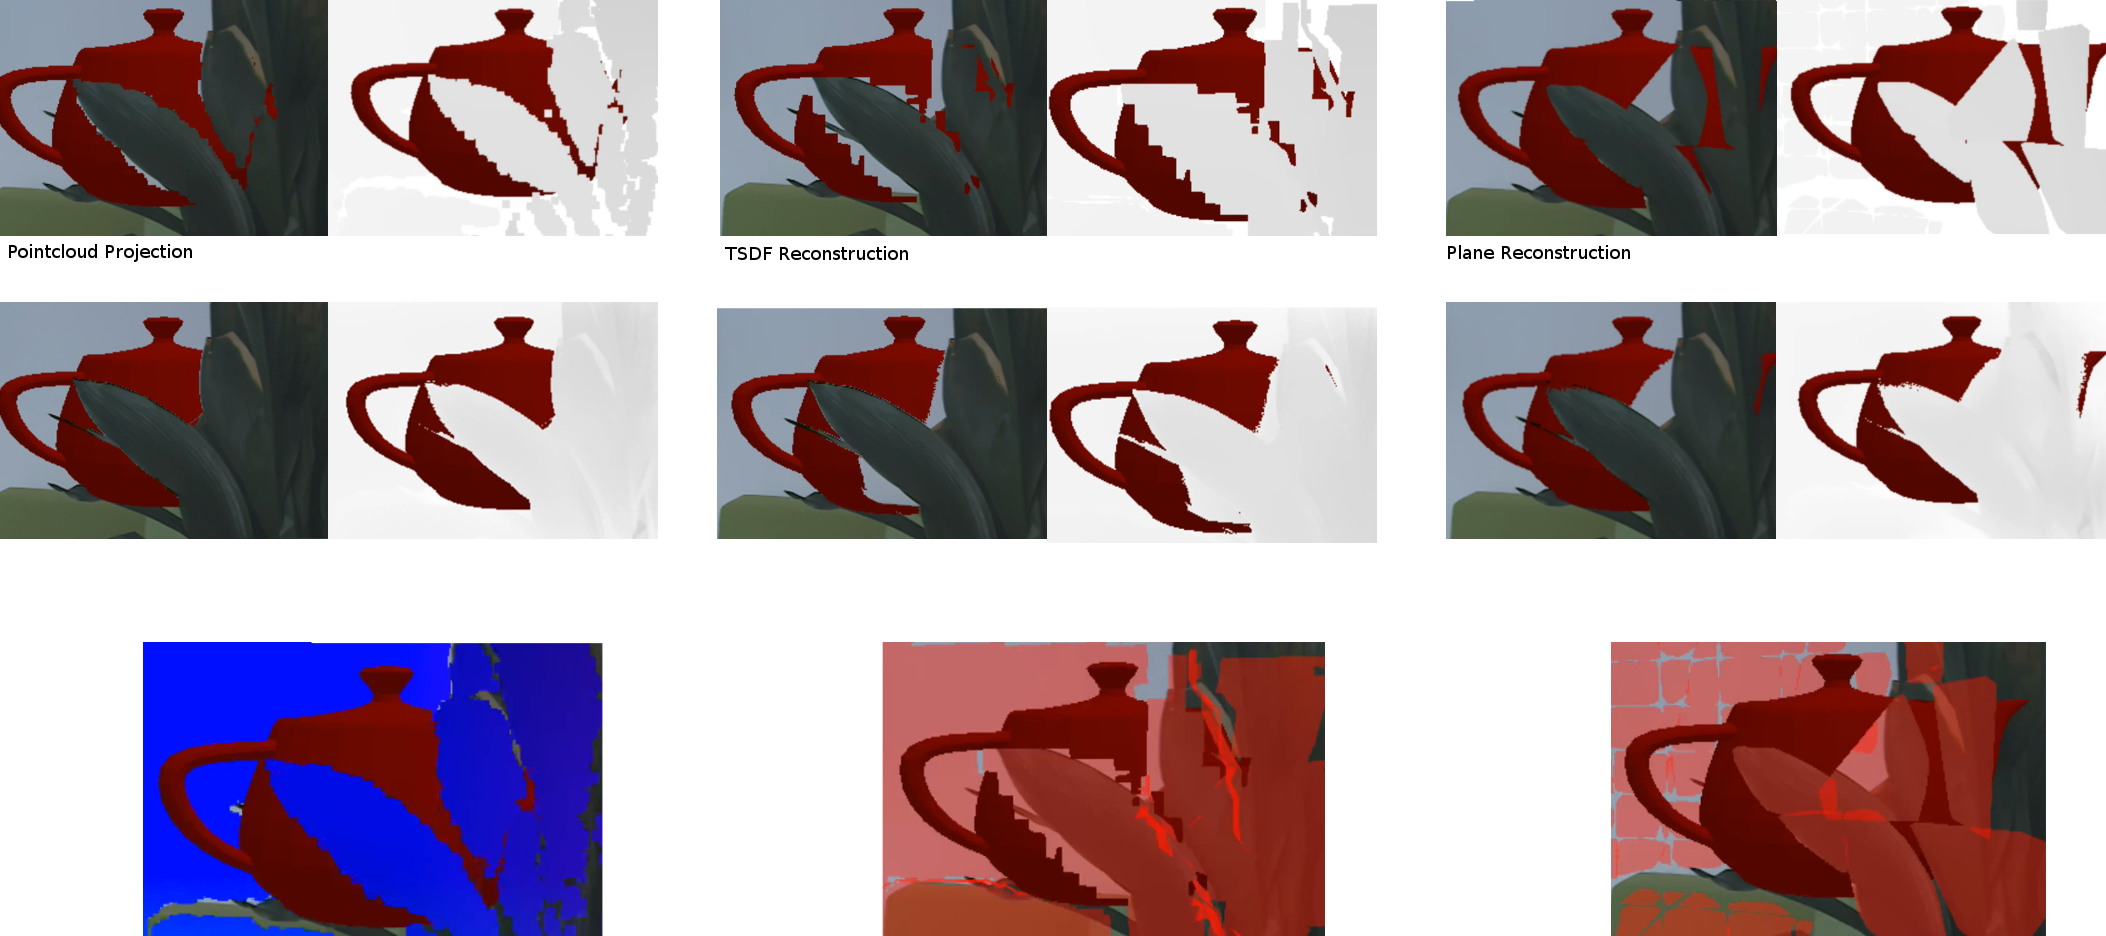
\includegraphics[width=1.0\textwidth]{content/images/evaluation/plant_occlusion.png} 
  \caption{Ergebnisaufnahmen aus der zweiten statischen Szene}
  \label{fig:plant_occlusion}
\end{sidewaysfigure}

\begin{sidewaysfigure}[h]
  \centering
	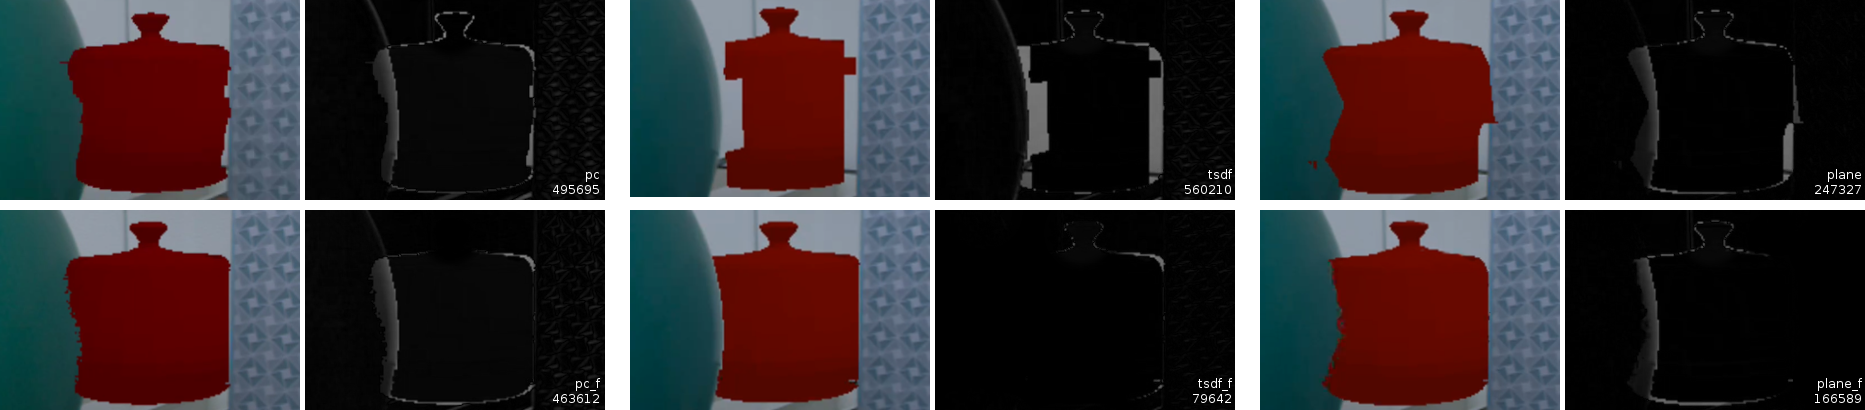
\includegraphics[width=1.0\textwidth]{content/images/evaluation/static_occlusion_results.png} 
	
\includegraphics[width=1.0\textwidth]{content/images/evaluation/spacer.png} 
	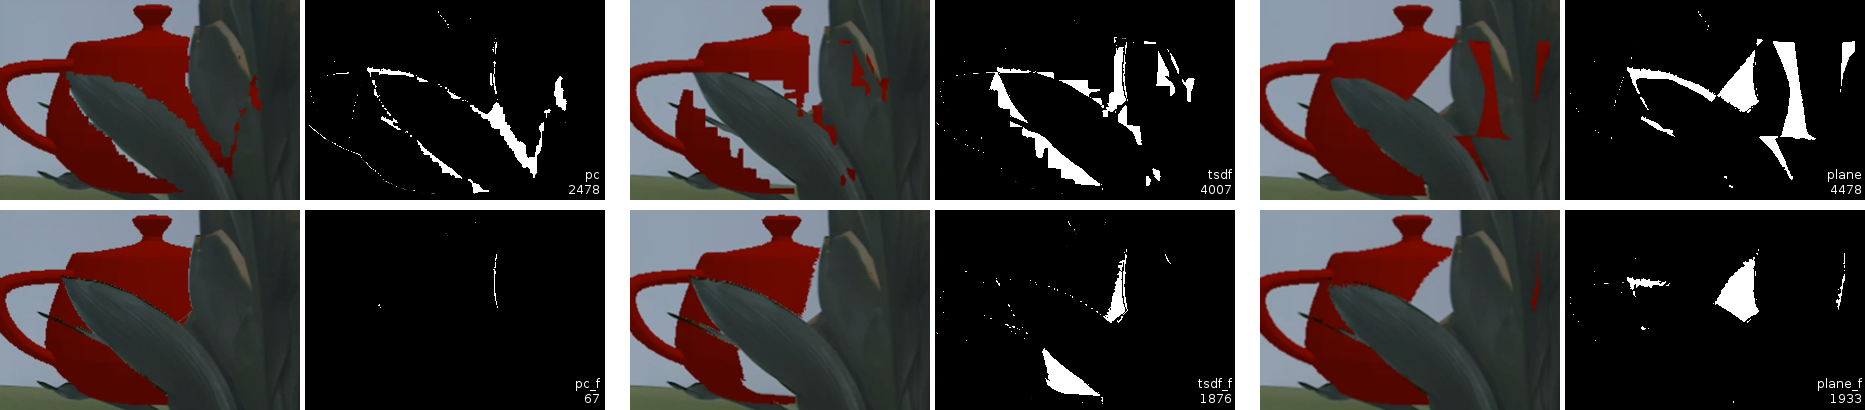
\includegraphics[width=1.0\textwidth]{content/images/evaluation/plant_occlusion_results.png} 
  \caption{Differenzbilder der Verfahren in ersten (oben) und zweiten Szene (unten)}
  \label{fig:static_occlusion_results}
\end{sidewaysfigure}



\addcontentsline{toc}{chapter}{Bibliography}

\bibliography{main}        
\bibliographystyle{natdin} 

\end{document}

